\chapter{The Experiment}

\section{Setup}

\subsection{Hardware}

All the tests were conducted on a laptop with a commodity processor
(Intel\textregistered Core\texttrademark $\,i5$ at $2.40$GHz). In
order to enforce serial execution \footnote{We are talking about BLAS
  or LAPACK; as the high level algorithms used were serial.}, even
when low level libraries attempted multi-threading, we used the Linux
\emph{taskset} command. The laptop has $8$Gb of RAM, but only 512Mb
were used on each experiment (and only for dense matrix algorithms;
sparse ones used much less). \\

\section{Data Preparation}

\subsection{The actual data}
We created 10 random matrices from application's domain data, using
the same encoding techniques they use in production; the sizes of such
matrices are in the range $[867,4500]$, so they fit in memory without
problem. \\

\subsection{Sparse formats}
Two sparse matrix formats were tested with Lanczos and LOBPCG
algorithms; namely the Compressed Sparse Row (CSR) and Compressed
Sparse Column (CSC) formats. For an overview of these and related
formats, in the actual context where we experimented with them, the
reader can consult \cite{johansson15}. While both formats showed
similar performance results, we prefer CSR because is the preferred
format used for the clustered eigenvalues removal pre-processing (see
below). 

\subsection{Avoiding clustered eigenvalues}

As we mentioned on previous chaper, clustered eigenvalues were a
headache for both Lanczos and LOBPCG; so we needed to do something
about them. By researching deeper why they were occurring, we found
that for the graphs behind the Laplacians produced by the
application, there was a common pattern: a disconnected graph with a
2-3 node small component, and the rest of the nodes in another big
component. \\

The theory says that for a disconnected graph of two components, the
first and second eigenvalues of the Laplacian will be zero (see
\cite{luxburg07}). In practice, what you get instead are two very
small numbers; and that is an extreme case of clustered
eigenvalues. They are very close to each other, because both try to
approximate zero. \\

The solution for this issue was to simply remove the already
disconnected small component; it makes sense given that ultimately,
the high level operation we want to perform on the graph is a
bipartition (thus, expectation is that the graph is connected). The
caveat was to compute the Strongly Connected Components (SCC) and the
new weights matrix quite efficiently, such that this pre-processing
did not become a performance penalty. The SCC computation can be done
efficiently (subsecond) with algorithm documented in \cite{pearce05},
for which we used the implementation available in SciPy; this
algorithm/implementation actually, is the reason why we prefer CSR
format over CSC (if the weights matrix is not passed in CSR format,
the routine takes much more time). \\

The recomputation of the weights matrix $W$ though, required bit more
of thought. It turned out that the CSR format is not very friendly
with row/column removal operations (which we need to do, in order to
simulate that nodes got removed from the graph). Based on an
StackOverflow post \cite{alim15}, we took the idea of using an
intermediate sparse sparse format (COO) which allows for faster
column/row removals; but at the same time, it also allows for fast CSR
conversion. The current StackOverflow post has an even faster option
published now, but the Python code below was good enough for our
experiments (it showed an overall time of $1.2$ secs for the biggest
matrices). \\

    \begin{lstlisting}
def split_cc_sparse2(W, cclab):
    idx_del = np.nonzero(cclab)[0]
    keep_row = np.logical_not(np.in1d(W.row, idx_del))
    keep_col = np.logical_not(np.in1d(W.col, idx_del))
    keep = np.logical_and(keep_row, keep_col)
    W.data = W.data[keep]
    W.row = W.row[keep]
    W.col = W.col[keep]
    W.row -= np.less.outer(idx_del, W.row).sum(0)
    W.col -= np.less.outer(idx_del, W.col).sum(0)
    k = len(idx_del)
    W._shape = (W.shape[0] - k, W.shape[1] - k)
    return W
    \end{lstlisting}

The snipet above works as follows: the argument
\emph{cclab} contains the node labels for the components, namely $0$ and $1$
for the big and small ones. Our goal is to eliminate the nodes with
label $1$ from the weights graph $W$. For that, that lines $1-8$
shrink first the index and data arrays (after removal of unwanted
columns/rows); lines $9-10$ eliminate the potential gaps on the
indices and finally lines $11-12$ truncate the $W$ to the new
size. The key idea is to do all the operations in terms of the NumPy
array primitives, which are quite efficient. 
    
\section{Results}

Though the laptop was idle at the time of the experiments, we captured
execution times as averages out of 100 executions (for each
algorithm/matrix combination). The graph below shows the results
obtained by encoding the matrices in CSR format. We present a
two-dimensional graph, with the X-axis representing the matrix size
and the Y-axis the average execution time in seconds. 

\begin{figure}[H]
  \centering
  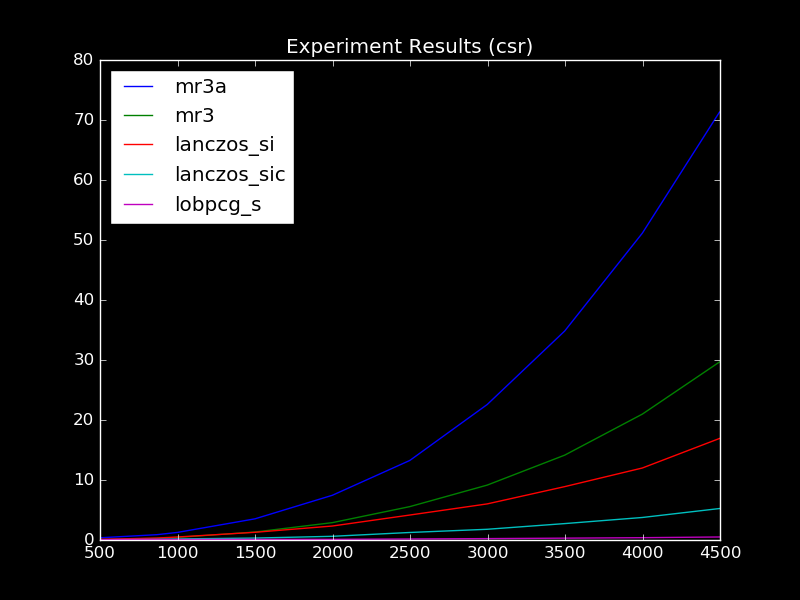
\includegraphics[width=11cm,height=8cm]{results-csr}
\end{figure}

The CSC results are basically the same, except for a sharp increment of 300
seconds for the $mr3a$ line (MRRR algorithm against biggest matrix):

\begin{figure}[H]
  \centering
  \includegraphics[width=11cm,height=8cm]{results-csc}
\end{figure}

We can perceive though, that the rest of the lines behave quite the
same, as the following graph shows:

\begin{figure}[H]
  \centering
  \includegraphics[width=11cm,height=8cm]{results-csc-wa}
\end{figure}
